\chapter{IOSharp}\label{C:IOSharp development}
In this chapter it will be explained how was defined and architected, designed and implemented the core of IOSharp, disaggregating the different parts and explaining each one.
\\
\\
First of all, it will be explained the project design evaluating the two options at project definition, then the implementation is explained for the different I/O ports and protocol standards used in this project. Finally, it is explained how has been done the port mapping to work between different boards and devices.

\section{Planning the development}\label{S:IOSharp-Design}
At the beginning of the project, the development was focused on a tiny Linux board called Raspberry Pi. This device was designed by Raspberry Pi Foundation in England taking in mind the kids around the world introducing them in computer science. It is an interesting board for its features like basic I/O through GPIOs, \gls{SPI} for serial peripheral communication, \gls{I2C} and UART interface also for transmissions between external components and the device itself.
\\
In addition to the interfaces mentioned above, it also has some desktop interesting features like USB ports which, practically can accept any device that works on Linux (for instance a Wi-Fi, Bluetooth, ZigBee or any stick for wireless transmissions, HDMI for graphics and Ethernet for network communications). Apart from this I/O characteristics, it also mounts an ARMv6 (CPU) running at 700MHz on stock frequency along with 512MB of RAM, that is enough for normal desktop usage (surfing, emailing and office) and for embedded projects.
\\
\\
After choosing the target device, two implementation options were suitable for this project so each one was analysed. Each one has its own benefits and problems that are going to be explained in the following sections. Some options have been considered, as the use of a specific library designed for the Raspberry Pi which should provide high efficiency. Or develop the implementation in a way that could be executed in any device running a Linux Kernel which makes the project platform independent.

\subsection{Focused on Raspberry Pi}\label{SS:IOSharp-RPI}
Initially IOSharp was started focusing on the Raspberry Pi, so a search was done in order to find useful libraries for this project and one of the results was a native C library. This library gives control over all the features provided by the microprocessor integrated on the board which includes a wide range of \gls{GPIO} pins, different protocol communications like \gls{SPI} and \gls{UART}, and other features like \gls{PWM}.
\\
This method is interesting when achieving high performance on the programs is important, so using the library the CPU features are used on a low-level way by using the CPU registers. This normally let the programs run faster but the programs only work on platforms using the same CPU, or in other words, is a specific hardware implementation.
\\
The library written for the \gls{BCM2835} is the one that should be used in the case that a program has high performance requirements. The idea is to make calls from C\# to this library using a specific call methodology that will be explained on future sections on this thesis.

\subsection{Focused on Linux}\label{SS:IOSharp-Linux}
Thinking on a more wider way it could be interesting to make IOSharp available to much more devices or even real computers. This implies more developers using this software which can provide useful feedback that is interesting for the improvement and evolution of the library. Any computer running some kind of Linux Kernel should be able to use this software facilitating the usage of the the hardware features.
\\
The idea is to use C\# combined with C to generate cross-platform assemblies, which making use of Mono, can run practically on any Linux device, but this has a little drawback related with the performance. Mono is a virtual machine which executes .NET code (C\#), the implementation of this VM is not as good as the .NET framework on Windows so normally the performance of the programs running on it is not really good.

\subsection{Chosen implementation}\label{SS:IOSharp-choosen}
Finally the chosen strategy was to use the Linux approach because it offers the appropriate tools like the \verb!spidev.h! to manage the SPI or even the GPIO mappings through the \gls{SYSFS}. To use any of this features the only requirement is that the necessary modules must be loaded into the Kernel.
\\
Micro Framework natively offers the required classes to configure the port mapping according to the pins and devices of the underlying hardware.
\\
Along with the C\# implementation, a C library will be written to interact with the functions provided by the Linux Kernel to control the \gls{SPI} and the \gls{GPIO}s.
\\
In short, IOSharp will be able to run in any platform that uses Linux such as the Raspberry Pi, a Cubieboard or even a standard desktop.

\section{Implementation}\label{S:Implementation}
In the following sections it will be explained how has been carried out the implementation of the IOSharp library. As a summary IOSharp works as Micro Framework but on a high level basis, so it is not a complete port of the original, instead of this it uses C\# to implement the same functions which are exposed by the framework. In this case, the original source code has been downloaded from \url{http://netmf.codeplex.com/}. From the folder \verb!\Framework\Core\Native_Hardware! can be obtained the necessary files to implement at least the GPIO and the SPI port along with the files for port mapping or event UART. The native files make use of internal implements, so when a method which does an internal implement, is called the virtual machine will take the call and process the function internally. IOSharp instead of implementing the virtual machine implements the functions as a normal method (opening and closing the brackets and inserting the code inside the method).
\\
\\
The final implementation of IOSharp should look like the following figure.
\begin{figure}[H]\begin{center}
 \centering
  \captionsetup{justification=centering}
  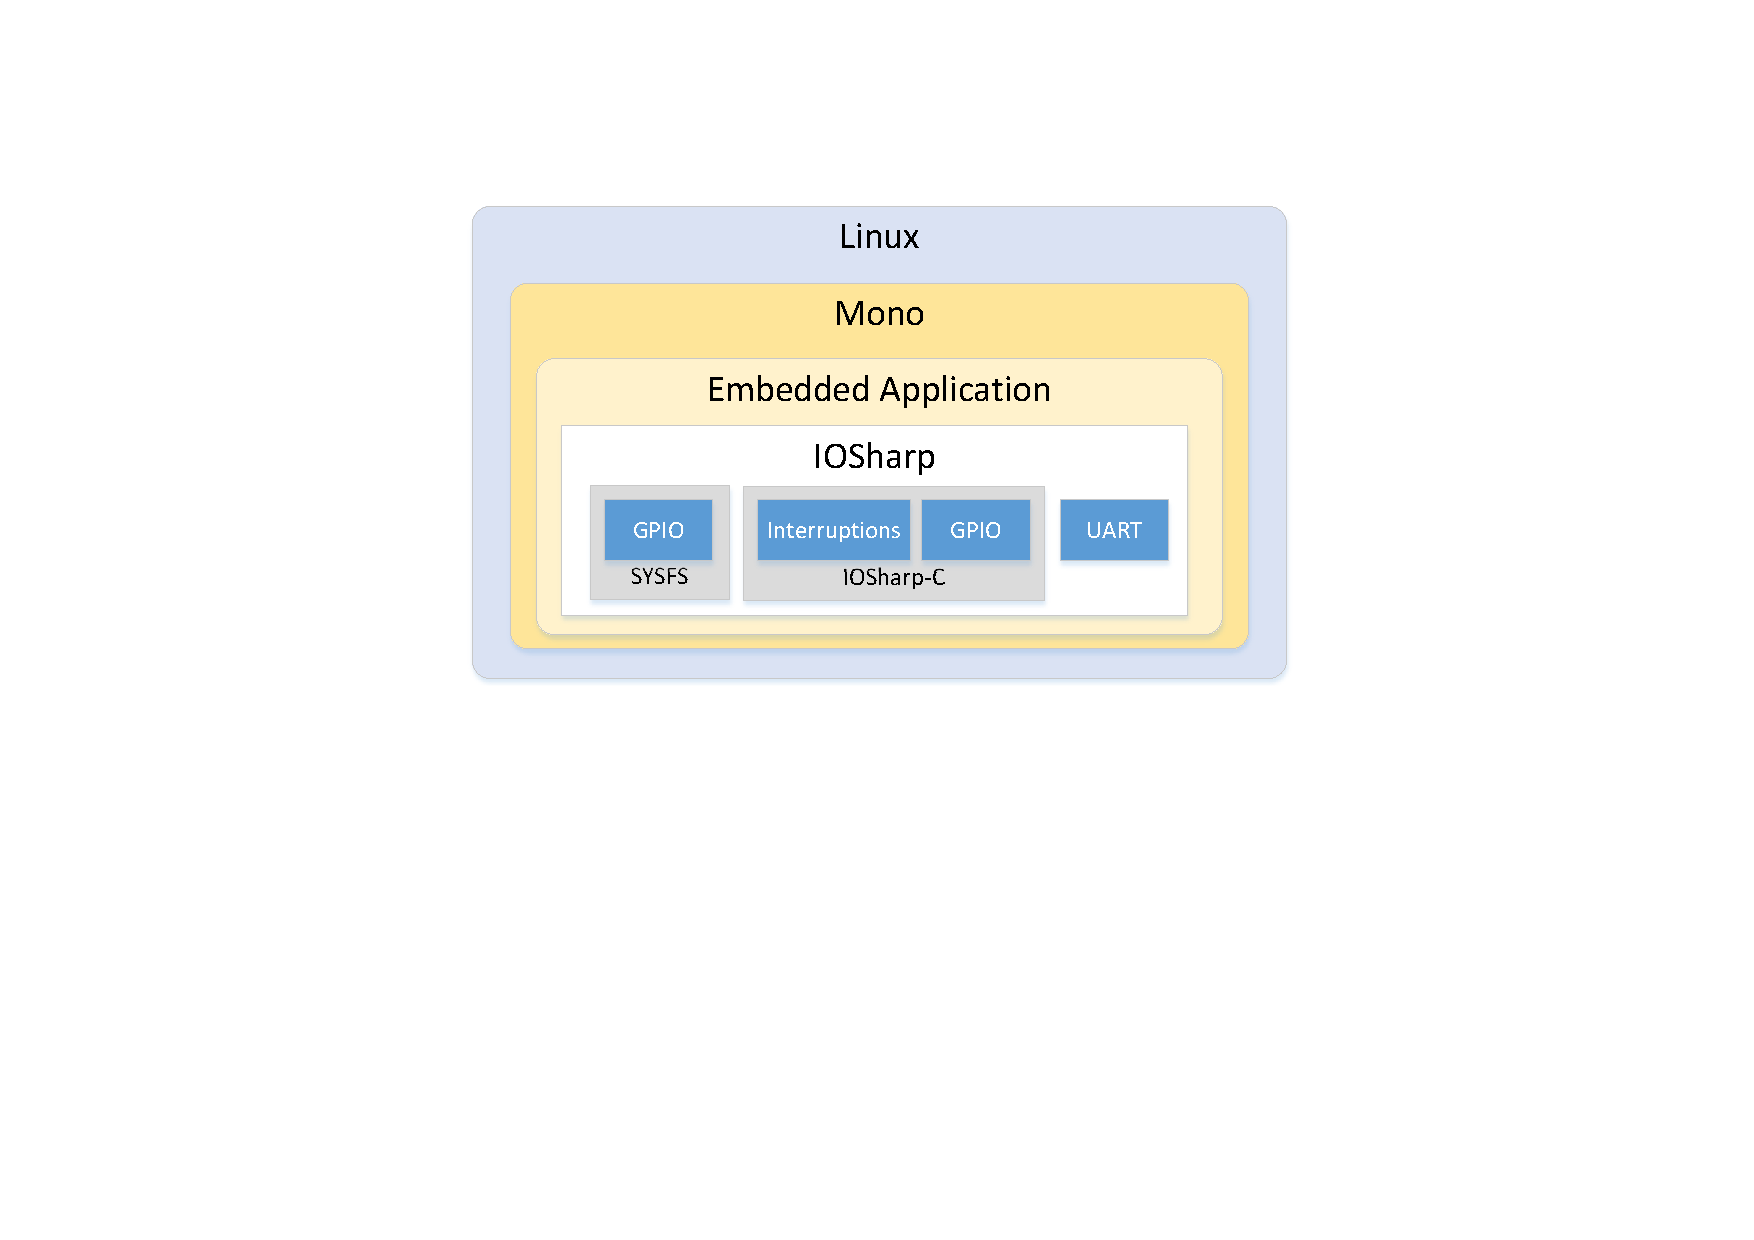
\includegraphics[scale=0.75]{pictures/iosharp/iosharp-schema2}
  \caption{Representation of the IOSharp \label{fig:interrupt-schema}}
\end{center}\end{figure}

\subsection{GPIO}\label{SS:GPIO}
GPIO acronym stands for General Purpose Input Output which are Ports on systems that are capable of generating an output or reading an input with a certain level of voltage. Normally embedded systems work at 3.3V, but low power devices can work at 2V.

\subsubsection{Implementation Options}\label{SSS:Implementation-Options}
In order to implement the GPIO ports in Micro Framework, it will be used the \verb!IOPorts.cs! file which contains the structure for Input, Output, Tristate and Interrupt ports. The first three will be explained in this section whereas the interrupt port will have a dedicated one.
\\
The GPIOs in Linux can be controlled in several ways. The most common and simple is to use the \gls{SYSFS}, which stands for a set of directories with readable and writeable files representing the ports of the CPU. On the other hand, the Linux kernel also provides a library to control the pins.
\\
The decision must be done between these two systems. In order to use any of this solutions the GPIO module must be loaded into the kernel. Many desktop Linux distributions have GPIOs disabled and that's why the kernel must be recompiled enabling this feature.
\\
In case of Linux operating systems designated for embedded devices, for example the Raspberry Pi or CubieBoard, they will have the I/O Ports enabled by default.
\\
It is interesting to point that Android is capable to use GPIO ports. Although it cannot seem an interesting feature nowadays, android is everywhere and can run in many devices, so this is another reason to try to fetch this sector in future versions of IOSharp.

\subsubsection{Using GPIO from SYSFS}\label{SSS:IOSharp-GPIO-SYSFS}
Since each solution can be used in this project and both are available in any Linux it was decided to use the SYSFS access because it is much easier to use and test the implementation. It only requires having read/write access to a certain set of files and directories and by reading or writing in this ones is possible to change the port states.
\\
\\
As it was said before, in SYSFS the control of the GPIOs is carried by several files and directories located under \verb!/sys/class/gpio! directory. In this directory there are two files which are called \verb!export! and \verb!unexport!, the first one is used to enable a GPIO while the second one disables it. After enabling a GPIO a new folder is created representing the enabled port, for instance if port 2 is enabled, a folder called gpio2 will be created. Inside this new folder there are several files, the \verb!direction! file describes how port should work, if the desired function is as an input port an \verb!in! must be written in the file whereas \verb!out! is used for an output port. After setting the port direction the next relevant file is \verb!value! which is used to set the port state in case of an Output Port (write 0 for a state-low or a 1 for a state-high) or in case of an Input Port it will read the incoming value through the port.

\subsubsection{Implementing in NETMF}\label{SSS:Implementing-GPIO-NETMF}
Taking in mind that this implementation has to be done over the existing code extracted from the \verb!IOPorts.cs! file, is important to design how to do it properly, in this case a \verb!GPIOManager! has been created using a singleton pattern. This class will restrict the number of instantiations that a port can have in order to avoid problems on the hardware. The instance of this singleton is shared across all the code.
\\
This manager will be in charge of enabling, disabling and operating the different I/O ports. Apart from this it also controls if a port is instantiated to avoid problems related to instantiate two port types in a unique pin.
\\
The figure \ref{fig:gpio-uml} shows the UML diagram of the \verb!IOPorts.cs! file from Micro Framework. Each class uses the \verb!GPIOManager! to control the read/write functions and port creation.

\begin{figure}[H]\begin{center}
 \centering
  \captionsetup{justification=centering}
  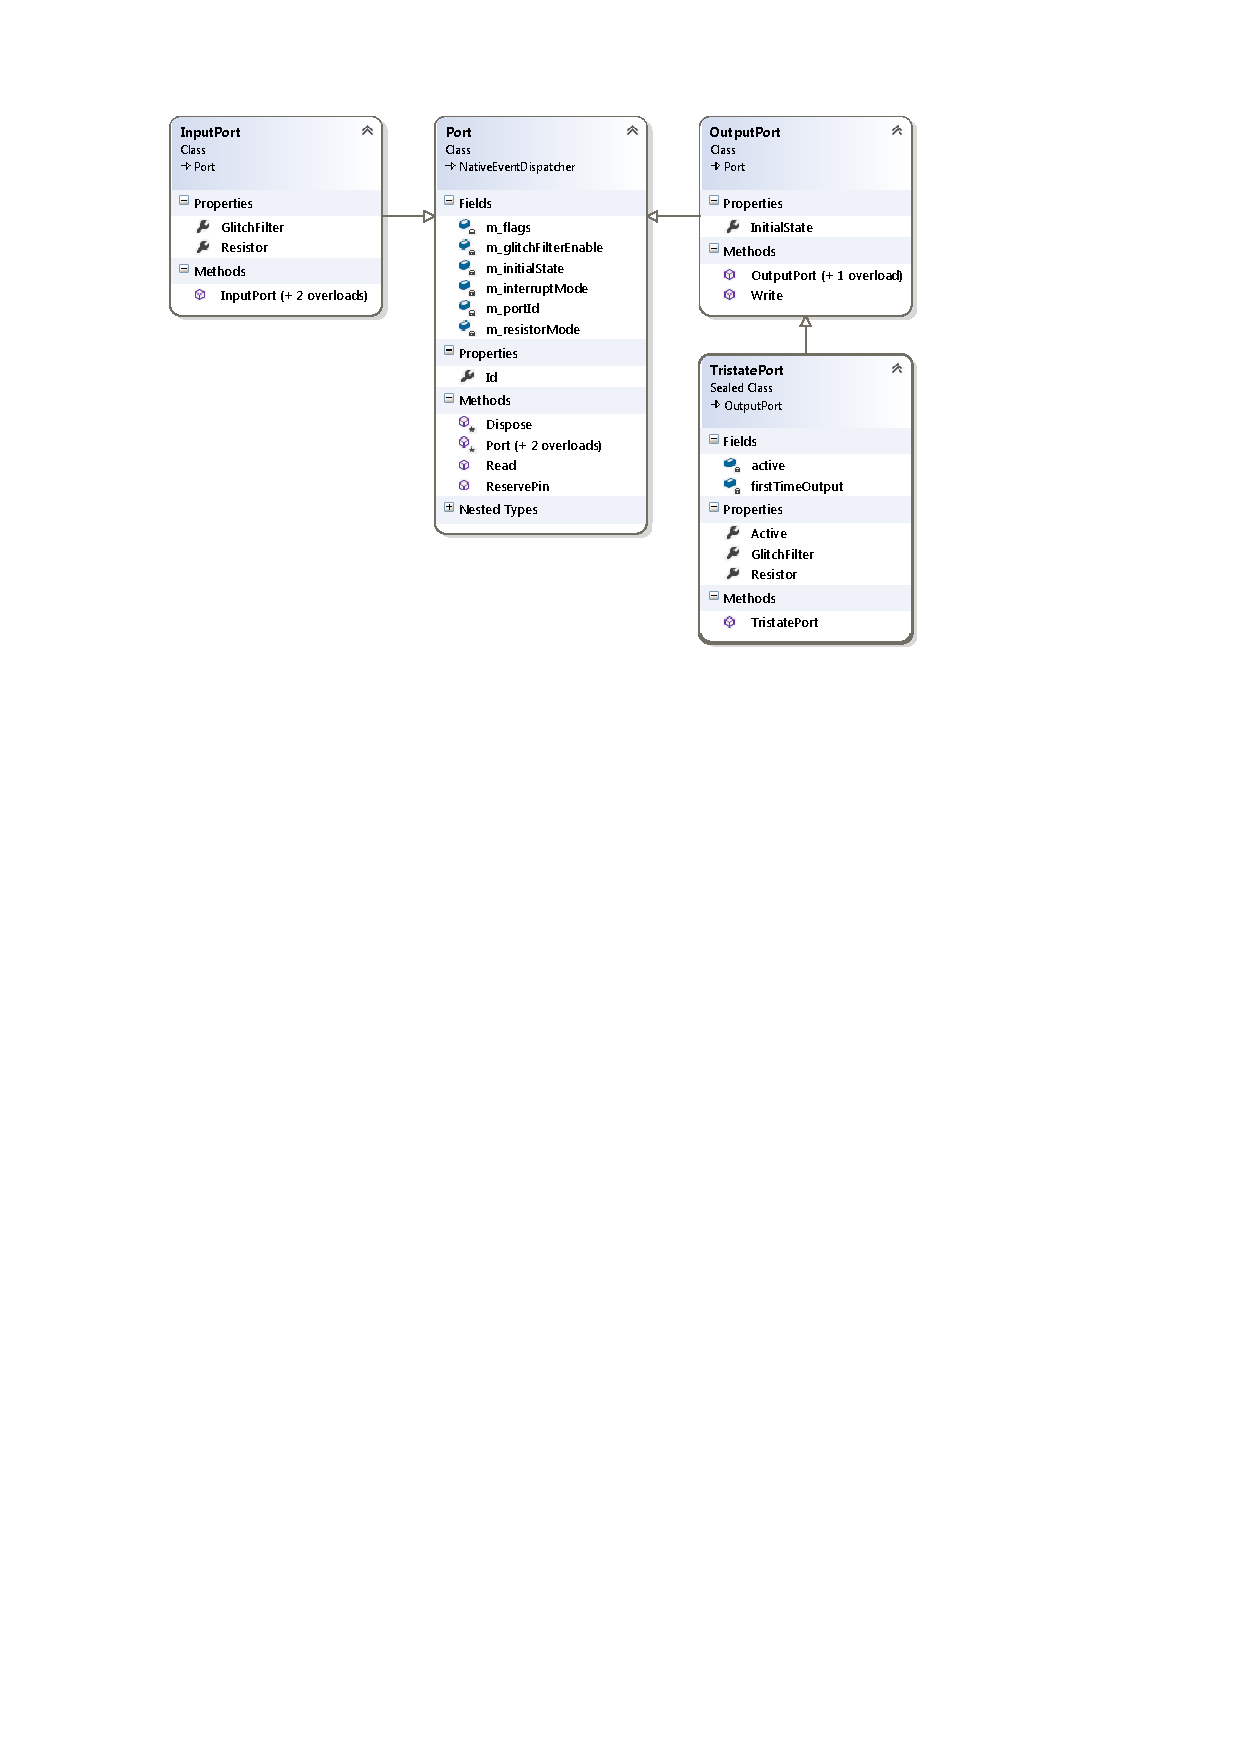
\includegraphics[width=1\textwidth]{pictures/iosharp/gpio}
  \caption{UML Diagram of NETMF Port and its inheritance \label{fig:gpio-uml}}
\end{center}\end{figure}

As is shown each port type inherits from the \verb!Port! object which implements the methods to enable or disable a port. \verb!Read! method is used to obtain the current state of the port i.e read an input value or even know the configured state in an output port. Finally the \verb!ReservePin! method permits to reserve a pin for a future usage.
\\
The \verb!InputPort! inherits from Port and it does not have any special method apart from its constructor which bases to the \verb!Port! class. 
\\
The \verb!OutputPort! which also inherits \verb!Port! implements a new \verb!Write! method which is used to write a state through the port (active-high or active-low).
\\
The \verb!TristatePort! inherits from \verb!OutputPort!. This port can change its functional work between an input or an output mode.

\subsection{Interruptions}\label{SS:IOSharp-Interrupt}
The interruptions which are needed for the interruptions that are required in the HomeSense program when using the \gls{SPI}. Although the \gls{BCM2835} supports native interruptions via \gls{IRQ} at the time of this project was developed the Raspberry Pi did not support GPIO interruptions using \gls{IRQ}.

\subsubsection{Designing the Interruptions}\label{SSS:IOSharp-Interrupt-Design}
The interruption system has been written in C in order to use a function called \verb!poll! which is commonly used by developers that want to detect GPIO interruptions using the SYSFS. The \verb!poll! function must be configured to wait and block until certain events occur on a \gls{FD} corresponding to a GPIO port enabled on the SYSFS. This function is configured to wait and block the program execution until the a \verb!POLLPRI! event on the \gls{FD} is detected. This event will be triggered by the OS when the file had urgent data to be read. Poll function will dectect the event and then will proceed with the following instructions to read different parameters from the port (i.e. the port state). Then, in C\# a delegate pattern will be used to notify to the upper layers of the program that interruption. The developer will configure the function which acts as the delegate by passing it to the \verb!OnInterrupt! property in the Interrupt Port.

\begin{figure}[H]\begin{center}
 \centering
  \captionsetup{justification=centering}
  \includegraphics[width=1\textwidth]{pictures/iosharp/interrupt-uml}
  \caption{UML Diagram of NETMF Interrupt Port \label{fig:interrupt-uml}}
\end{center}\end{figure}

\subsubsection{Platform Invocation Services}\label{SSS:IOSharp-Interrupt-PInvoke}
In C\# is possible to invoke external libraries which are not written in the same language. In this case, the library used for the interruptions is written in C and it will be compiled into a shared library making it available to any program, or in this case, IOSharp.
\\
\\
Take a look into the appendix \ref{S:appendices-libraries-types} to know more about the different library types.
\\
\\
P/Invokes in .NET make use of dynamic loaded libraries in order to use the contained functions. The implementation difficulty of a P/Invoke increases on how complex is the function to be called regarding its parameters, for basic type parameters such us \verb!int!, \verb!long!, \verb!byte! is really simple to make a P/Invoke call, but when passing object parameters things get much more difficult because this requires doing marshalling in this objects. Marshalling is similar to serializing but maintaining some information related to the object. The marshalling is used to pass from managed to unmanaged code and sometimes is impossible without using intermediate structs as interchange objects.
\\
\\
Below are shown the important parts of the implementation of this library and then how P/Invoke is done in C\# code.
\\
This first block shows the function which is used to detect the interruptions on the GPIOs. The interesting parts are commented explaining what they do or what some macros mean.
\begin{lstlisting}[language=C, caption={IOSharp.c - Polling function}]
uint64_t start_polling(int pin) {
    struct pollfd fdset;
    int nfds = 1;
    int gpio_fd, timeout, rc;
    char * buf[MAX_BUF], c;
    int len, count, i;
    long t;

    // Get the File Descriptor for the GPIO Port. See function on the Library.
    gpio_fd = gpio_fd_open(pin);

    // Clear any initial pending interrupts
    ioctl(gpio_fd, FIONREAD, & count);
    for (i = 0; i < count; ++i)
        read(gpio_fd, & c, 1);

    // Fill fdset which is a struct for pollfd which is used to describe the polling system.
    // In this case the File Descriptor for the GPIO port is entered, and then the POLLPRI (Data Urgent to Read) is configured as the event type.
    fdset.fd = gpio_fd;
    fdset.events = POLLPRI;

    read(fdset.fd, & buf, 64);

    // Start polling the File Descriptor. POLL_TIMEOUT variable contains (-1) which stands for infinite blocking until event.
    rc = poll( & fdset, 1, POLL_TIMEOUT);

    // Close the GPIO Port. See function on the Library.
    gpio_fd_close(gpio_fd);
    return t;
}
\end{lstlisting}
After writing the function this must be exposed using a header file which is shown below.
\begin{lstlisting}[language=C, caption={IOSharp.h - Header file for the library}]
#ifndef IOSHARP_H_INCLUDED
#define IOSHARP_H_INCLUDED

// Define the polling function
uint64_t start_polling(int pin);

#endif
\end{lstlisting}
And finally this block represents how is done a P/Invoke in a C\# program. The function is exposed using a \verb!public static extern! and then an attribute is attached which corresponds to the \verb!DllImport! which specifies the shared library to call.
\begin{lstlisting}[language=CSharp, caption={GPIOManager.cs - P/Invoke section}]
// The function which calls the external function
private void Listen(object obj) {
    ThreadHelper th = (ThreadHelper) obj;
    while (true) {
        int pin = (int) th.Pin;
        // Call the function. See down.
        ulong cback = GPIOManager.start_polling(pin);
        th.Callback(4, (uint) 0, DateTime.Now);
    }
}

// External function represents a function on an external library, in this case the library is the libIOSharp-c.so. The function naming and functions parameters are equal to the original function, but taking into account that a ulong in C# is a uint64_t on C.
[DllImport("libIOSharp-c.so", CallingConvention = CallingConvention.StdCall)]
public static extern ulong start_polling(int gpio);
\end{lstlisting}

\subsubsection{Final implementation}\label{SSS:IOSharp-Interrupt-Implementation}
The program flow is shown on Figure \ref{fig:interrupt-schema} which represents the steps that IOSharp does for the interruptions system. The Interrupt Port inherits from Input Port as Figure \ref{fig:interrupt-uml} shows.
\begin{figure}[H]\begin{center}
 \centering
  \captionsetup{justification=centering}
  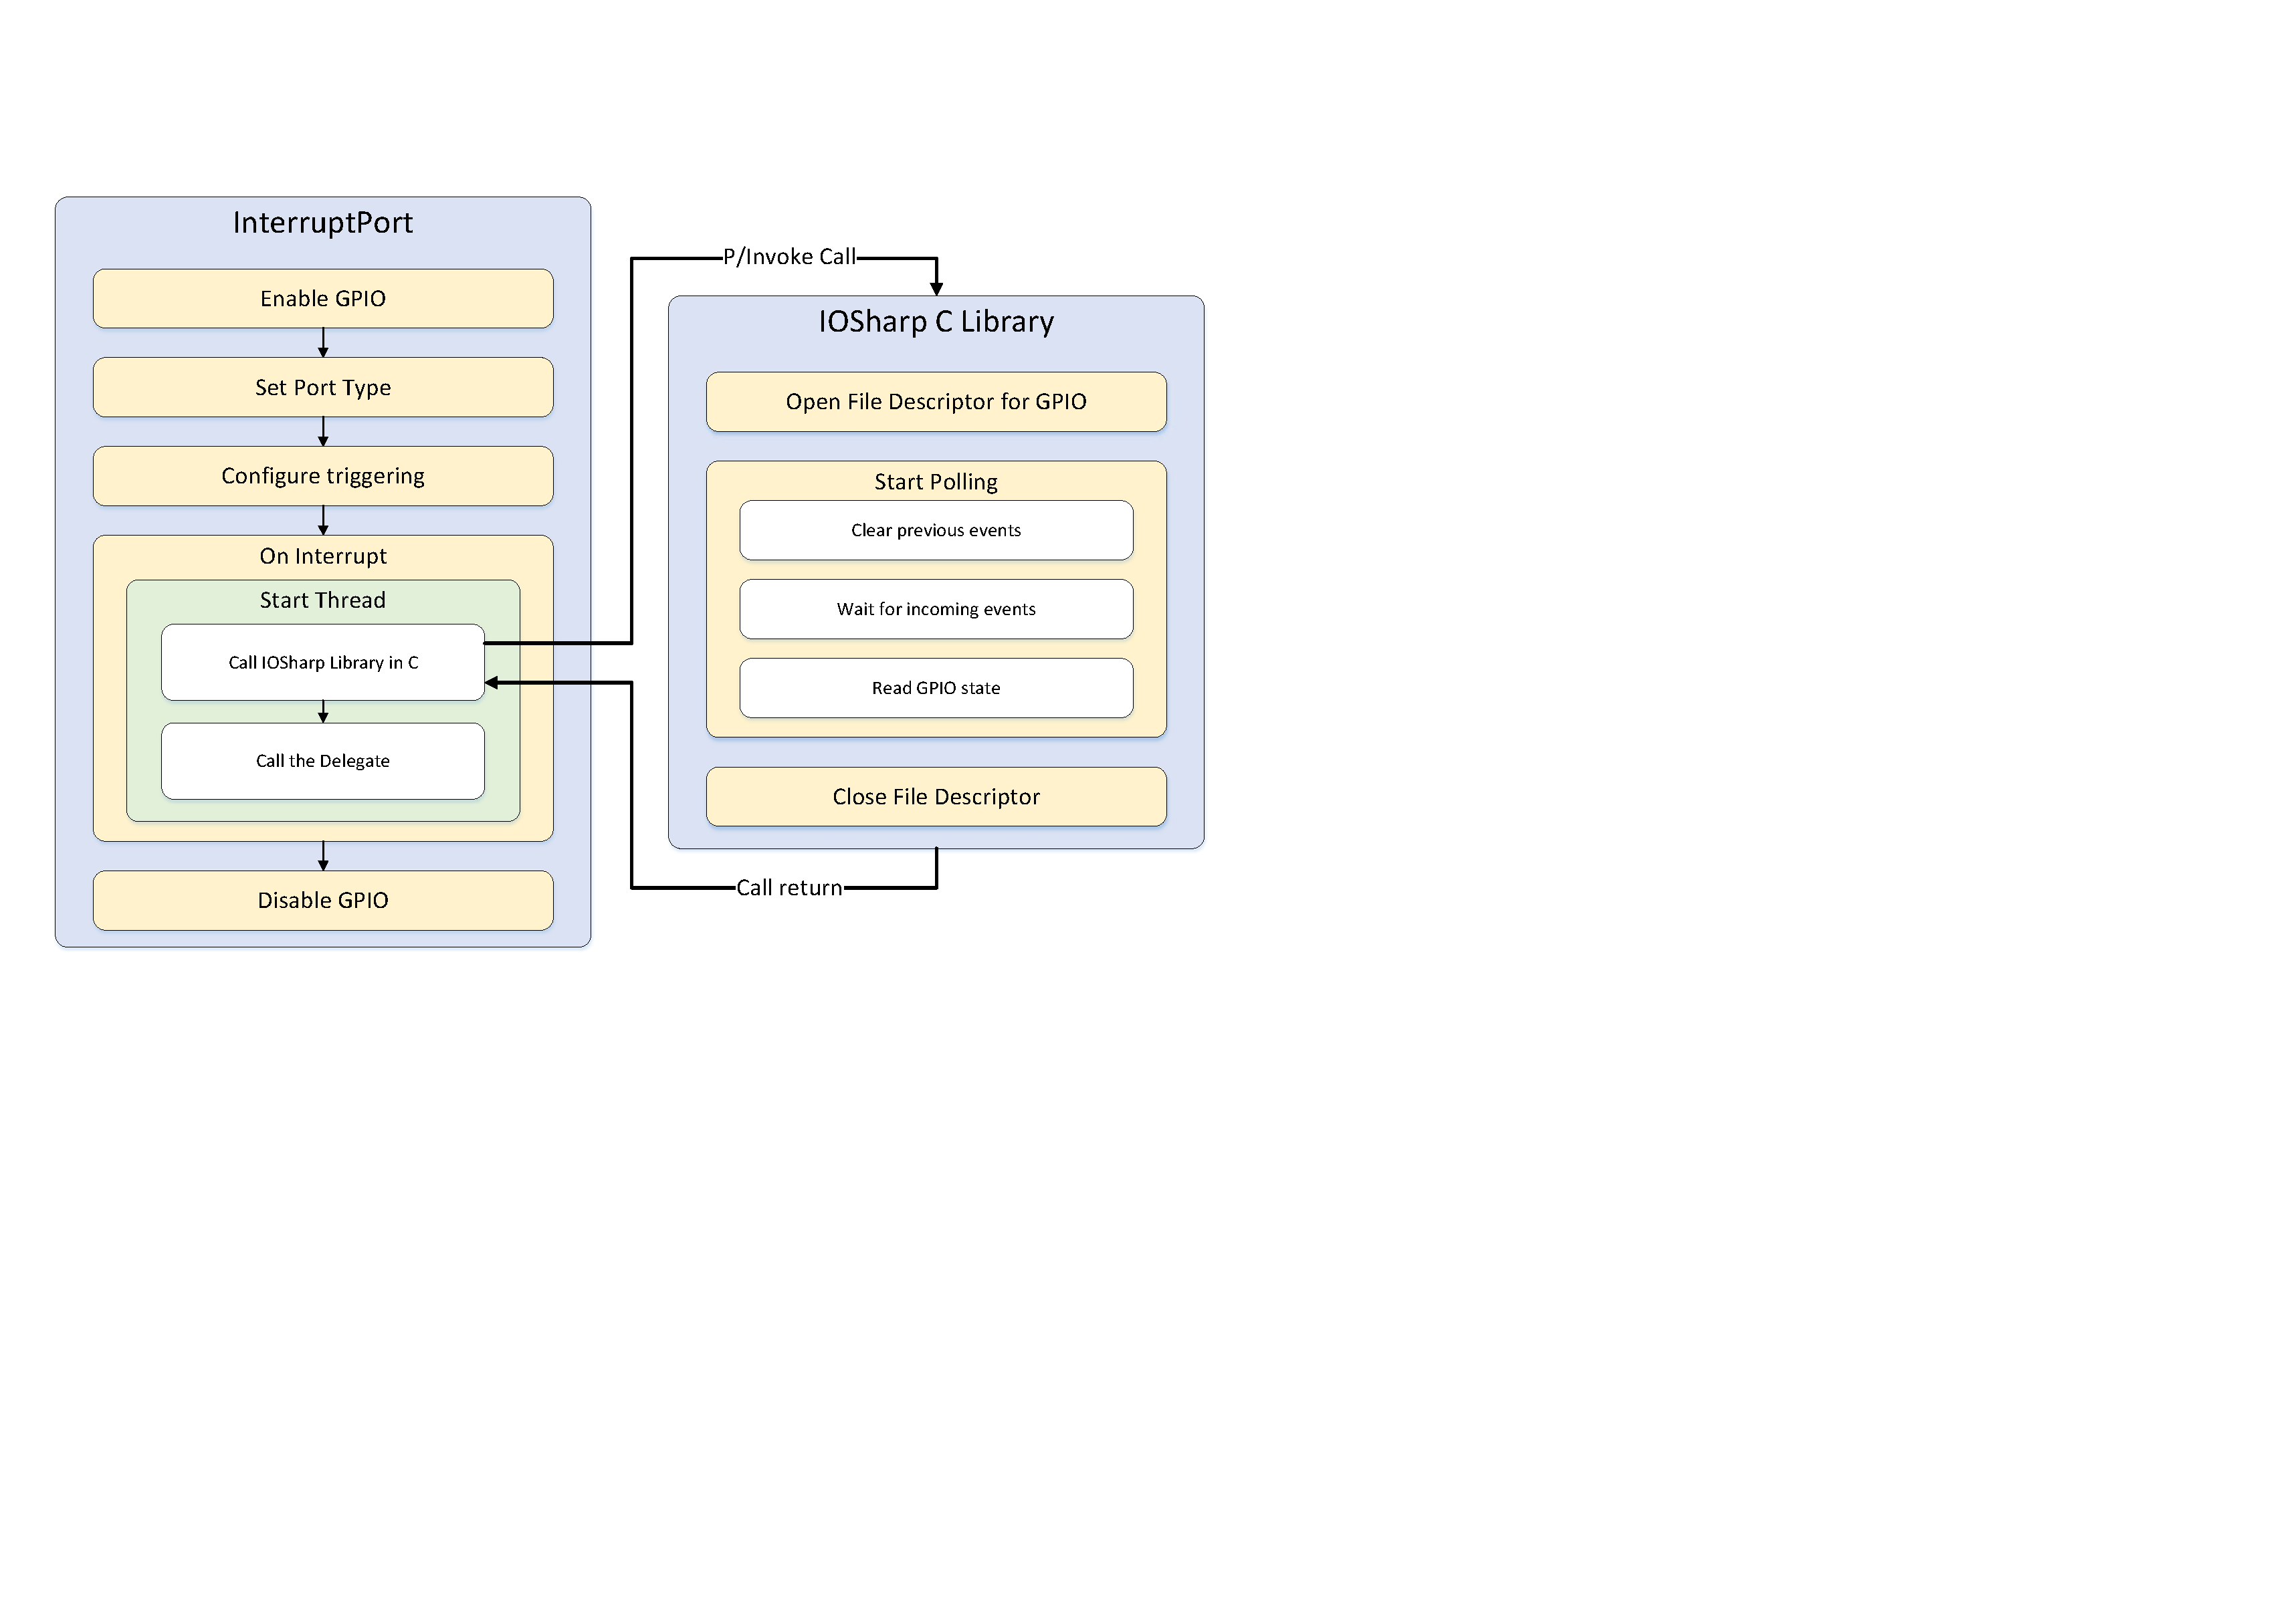
\includegraphics[width=1\textwidth]{pictures/iosharp/interrupt-schema}
  \caption{Representation of the Interrupt Port flow \label{fig:interrupt-schema}}
\end{center}\end{figure}
The idea is to do the exact same steps like the other ports do, the port enabling is done by the Port implementation which is the base class for Interrupt Port, then the port type is set to be an Interrupt Port, after doing this is the triggering must be configures. Micro Framework boards usually support four kinds of interruptions whereas Linux supports a few less, in the table \ref{T:Interrupt-Trigger-Types} are shown the ones that are supported. It is important to know that the edges are the point where the read state changes from one level to the other one. The Level is used when the state is maintained several time without changing.

\begin{table}[htb]
\begin{center}
\begin{tabular}{|c|c|c|}
\hline
{\bf Trigger Type} & {\bf Micro Framework} & {\bf Linux}  \\ \hline \hline
InterruptNone        & X    & X       \\ \hline
InterruptEdgeLow        & X    & X       \\ \hline
InterruptEdgeHigh        & X    & X       \\ \hline
InterruptEdgeBoth        & X    & X       \\ \hline
InterruptEdgeLevelHigh        & X    &        \\ \hline
InterruptEdgeLevelLow        & X    &        \\ \hline
\end{tabular}
\caption{Interrupt Trigger Types}
\label{T:Interrupt-Trigger-Types}
\end{center}
\end{table}

Like the GPIO the triggering is configured on the SYSFS on a file called \verb!edge! located inside of the enabled GPIO folder. This file can be configured on three different. \verb!EdgeLow! interruptions require the word \textit{falling} be written in that file, in case of \verb!EdgeHigh! \textit{rising} is used and finally \textit{both} is for \verb!EdgeBoth!.
\\
The polling thread works as an infinite loop P/Invoking to C and waiting for the call return, when this occurs the delegated function is called and this indicates that an interruption event occurred.

\subsection{SPI}\label{SS:IOSharp-SPI}
The \gls{SPI} is one of the important features to be implemented on IOSharp. This protocol is used in embedded systems to communicate boards and components in a Master-Slave way. It offers a full-duplex communication channel where the master and the slave can write and read at the same time. Normally this protocol accepts transmission frequencies in the range of 10 kHz to 100 MHz and in order to operate the master configures its clock using a frequency less or equal to the maximum frequency supported by the slave which wants to communicate.
\\
Figure \ref{fig:spi-modules} show how is used a SPI bus, a master device can have several slaves attached to its ports. The minimal system is composed by three ports which are the bus itself, the \gls{MOSI} is the channel where the Master device writes and from where Slaves read the written information. The \gls{MISO} is the channel where the Master reads the information that the Slave writes. The \gls{SCLK} is used to set the clock of the system between the Master and the Slave. Finally for each Slave it must be \gls{CS} in order to select the slave that must active during the transmission.
\begin{figure}[H]\begin{center}
 \centering
  \captionsetup{justification=centering}
  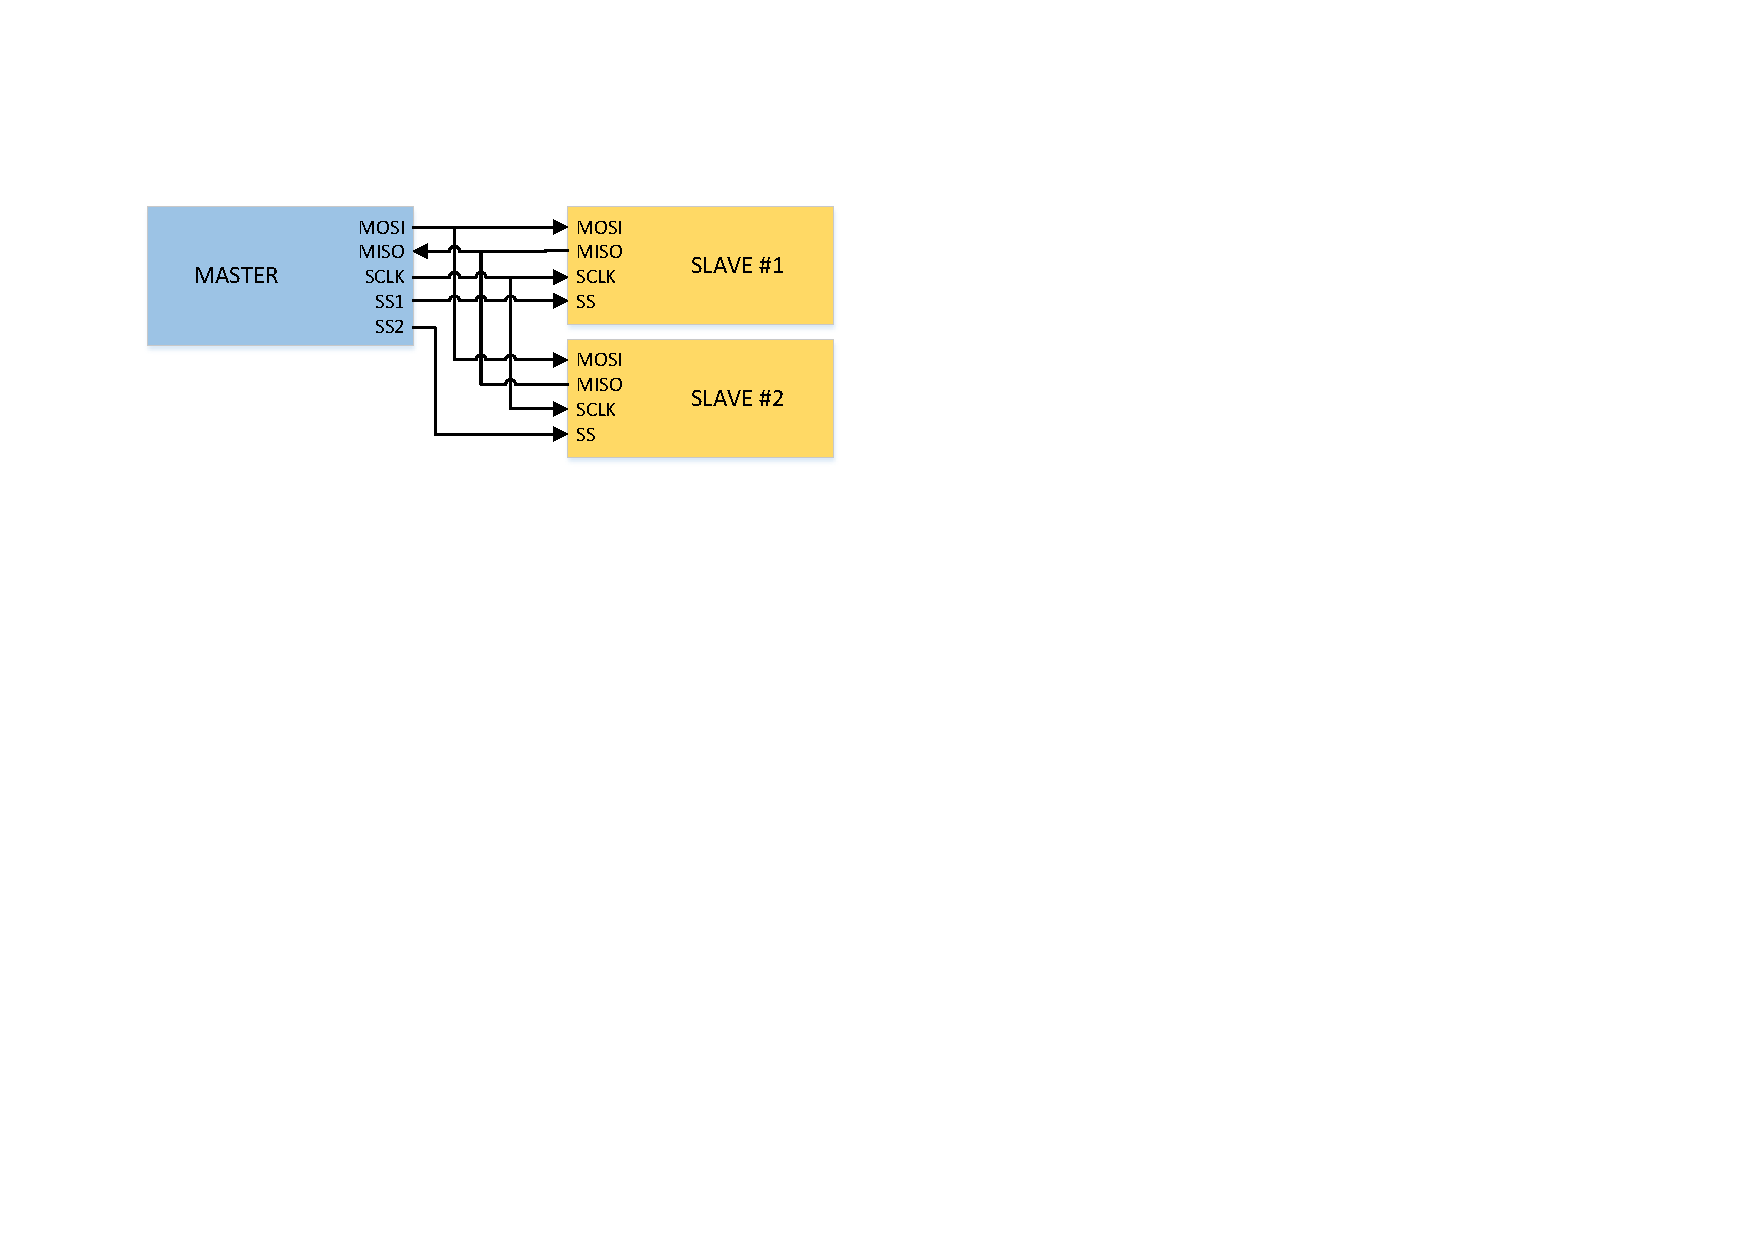
\includegraphics[scale=0.9]{pictures/iosharp/spi-modules}
  \caption{SPI bus setup with one master and two slaves \label{fig:spi-modules}}
\end{center}\end{figure}

\subsubsection{Designing the SPI}\label{SSS:IOSharp-SPI-Design}
The SPI implementation has been carried out like the Interrupt Port explained in the section \ref{SS:IOSharp-Interrupt}. In this case it has been used the Linux Kernel by using the \verb!<linux/spi/spidev.h>! library which makes the control of a SPI device very easy.
\\
SPI devices are mapped under \verb!/dev/! directory with a naming like \verb!/dev/spidevX.Y! the \verb!X! is an integer and represents the device (a CPU can have multiple SPI devices so this number will indicate the device number), then the \verb!Y!, also an integer, enumerates the \gls{CS} (SPI devices have multiple chip selects, so they can have more than one slave).
\\
\\
Before doing a transaction via the SPI this must be configured, first of all defining the operational mode. Modes are defined with the parameters Clock Polarity (CPOL) and Clock Phase (CPHA). Both are related to the sampling edge according to the clock (SCLK) used in the communication. The CPOL defines the polarity of the clock so the sampling will be done when de clock is in edge low or in edge high according to the configured parameter, CPHA defines in which phase the sample must be done. This concept is much easy to understand using the figure \ref{fig:spi-modes} which shows the different CPHA and CPOL options with the equivalent SPI modes required to be configured in the C library.

\begin{figure}[H]\begin{center}
 \centering
  \captionsetup{justification=centering}
  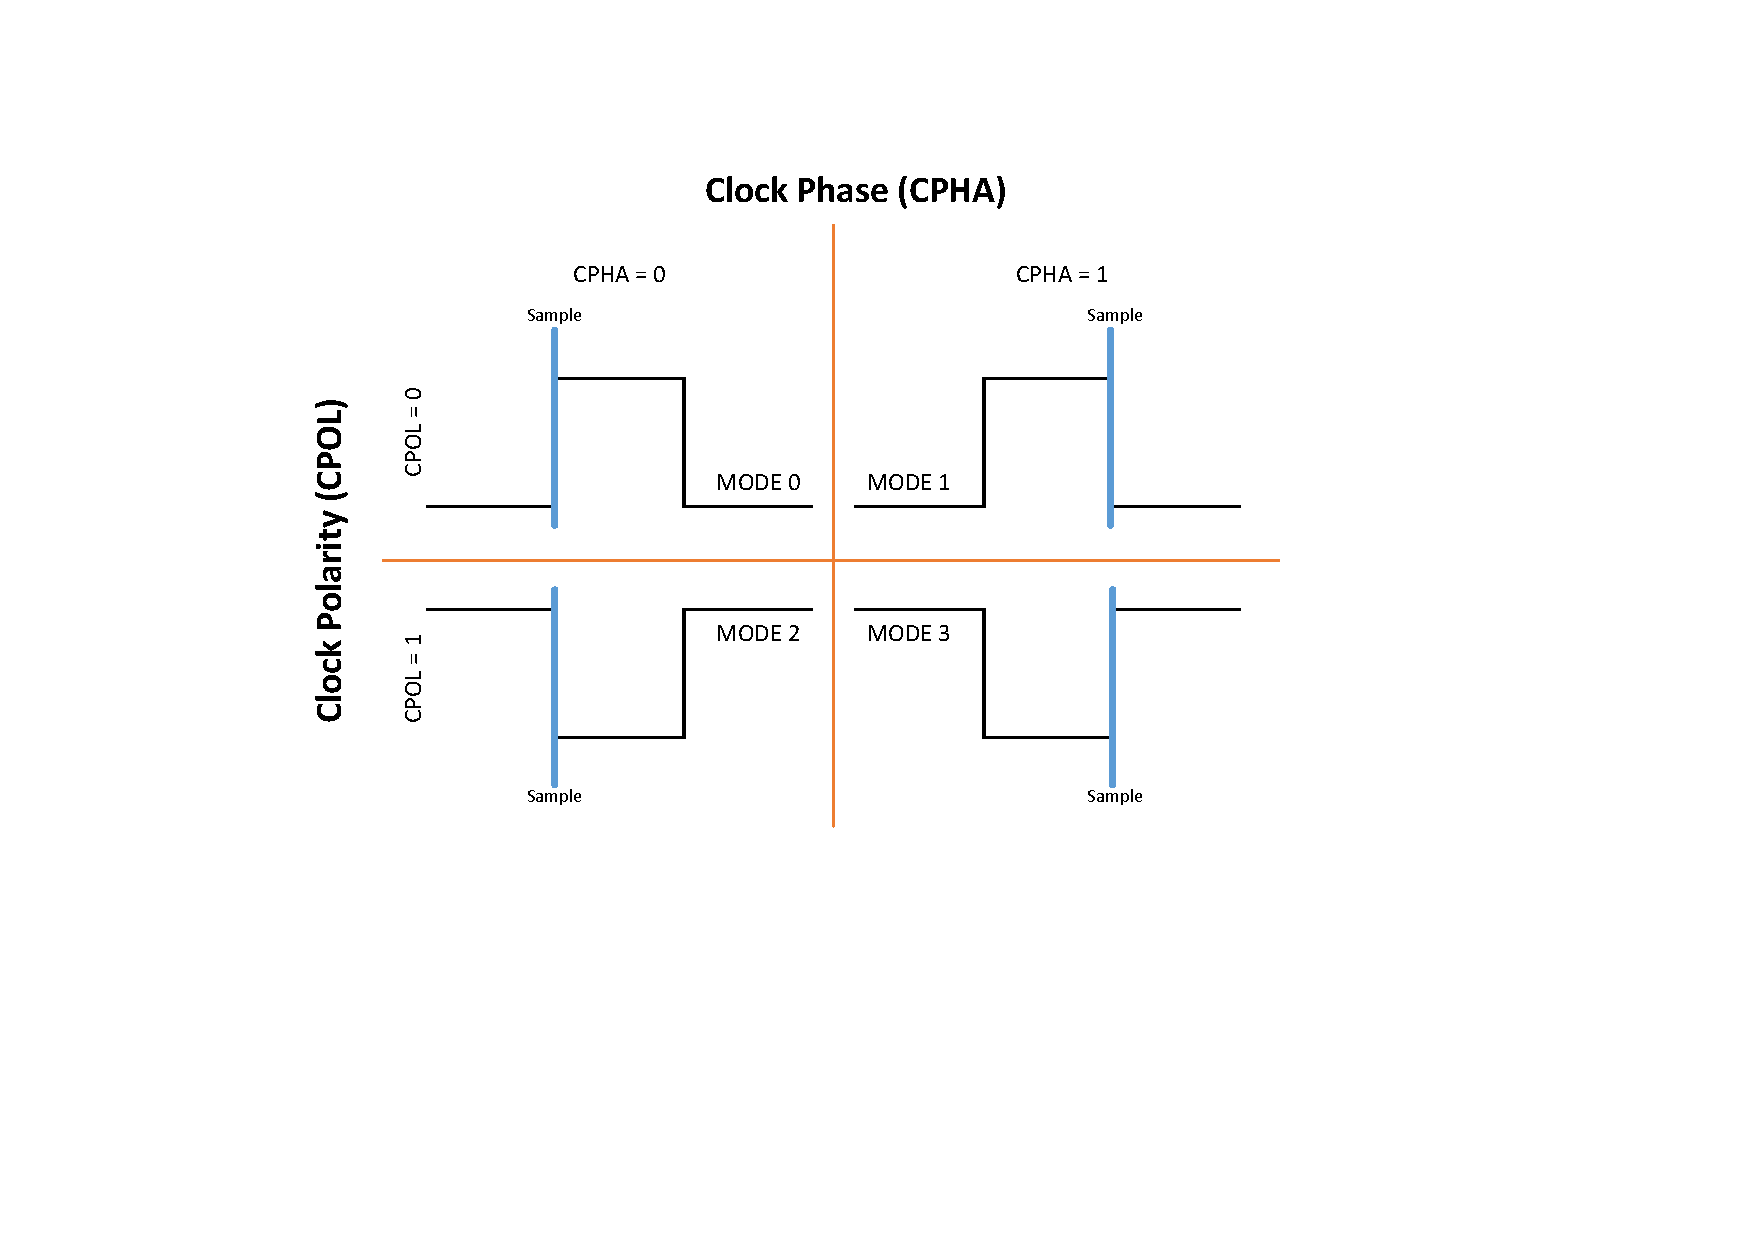
\includegraphics[width=0.7\textwidth]{pictures/iosharp/spi-modes}
  \caption{SPI modes are defined with the parameters "CPOL" and "CPHA" relatives to the data sampling acording to the System Clock (SCLK) state.\label{fig:spi-modes}}
\end{center}\end{figure}

This modes must be configured using the \gls{IOCTL} function passing the \gls{FD} according to the SPI device and the desired \gls{CS}, then the preprocessor macro \verb!SPI_IOC_WR_MODE! is used to specify which parameter will be configured, in this case its the SPI mode that has been explained before, the last parameter corresponds to another macro which defines the operational mode, the figure \ref{fig:spi-modes} shows each mode and the macro that must be passed to the \gls{IOCTL} function, this modes are \verb!SPI_MODE_0!, \verb!SPI_MODE_1!, \verb!SPI_MODE_2! and \verb!SPI_MODE_3!.

\begin{lstlisting}[language=C, caption={IOSharp.c - SPI Mode configuration}]
uint8_t mode;
  int ret;

//The mode variable can be SPI_MODE_0, SPI_MODE_1, SPI_MODE_2 and  SPI_MODE_3
  ret = ioctl(fd, SPI_IOC_WR_MODE, &mode);
  if (ret == -1)
    pabort("can't set spi mode");
\end{lstlisting}

Once the SPI mode has been configured a struct defining the transaction must be filled, the struct type of is \verb!spi_ioc_transfer! specified in the \verb!spidev.h! library. This struct contains different variables, the \verb!tx_buf! and \verb!rx_buf! are configured with the write and read. Apart from the buffers, the transmission length is configured using the variable \verb!len!. Then the delay is configured, this indicates how many microseconds the SPI driver must wait before starting the transmission, this is important because some slaves take some time between they are selected and they are able to communicate, this is configured using the \verb!delay_usecs! variable. Another parameter to configure is the clock by using \verb!speed_hz!. In order to deselect a device before a transfer, the parameter \verb!cs_change! must be true. Finally, to configure or override the wordsize of a transmission the\verb!bits_per_word! is used.

\begin{lstlisting}[language=C, caption={IOSharp.c - SPI struct configuration}]
struct spi_ioc_transfer tr = {
    .tx_buf = (unsigned long)writeBuffer,
    .rx_buf = (unsigned long)readBuffer,
    .len = writeCount,
    .delay_usecs = spi.delay,
    .speed_hz = spi.speed,
    .cs_change = spi.cs_change,
    .bits_per_word = 8,
  };
\end{lstlisting}

Once the struct is configured another ioctl call is done which makes the transfer it self. In this case, along with the \gls{FD} corresponding to the SPI device another preprocessor macro is passed as a parameter, this one is called \verb!SPI_IOC_MESSAGE! and must include the number of transfers that will be executed together, in case of IOSharp there is only one transfer per call, so the parameter will look like \verb!SPI_IOC_MESSAGE(1)!, finally the struct commented above is included in the ioctl call.

\begin{lstlisting}[language=C, caption={IOSharp.c - SPI transfer}]
// Pass the preprocessor macro and the spi_ioc_transfer struct.
ioctl(fd, SPI_IOC_MESSAGE(1), &tr);
\end{lstlisting}

\subsubsection{Implementation in C\#}\label{SSS:IOSharp-SPI-Implementation-CSharp}
After writing the library part in C is time to modify IOSharp to add the necessary calls to this library in order to make Micro Framework use the SPI in Linux. In this case the calls will be done in a similar way as it has been done in the interruptions (\ref{SS:IOSharp-Interrupt}). In this case some data will need to be serialized in order to pass the configuration of the SPI from C\# to C.
\\
Essentially the method will be do a P/Invoke from C\# in order to call the functions in the library. To facilitate the data exchange between the program and the library a struct is used, this contains the basic information in order to do the configurations explained on the previous section. This struct must be written in the header file of the library and also must be written in the C\# code. First of all the SPI implementation in Micro Framework is divided into two blocks, the first one represents the port configuration which is used to set the different properties that can be used with the SPI, for example the clock rate, the setup time of the slave, the SPI modes (CPHA and CPOL), etc. The second block, which is the SPI itself uses the configuration commented above to create an SPI instance, along with the required pins for the \gls{MISO}, \gls{MOSI}, \gls{SCLK} and \gls{CS}.
\\
When the SPI instance is created, the methods will be able to be used, basically there are different overloads of the \verb!Write! and \verb!WriteRead! methods, but all of them end calling the same internal function which will do the P/Invoke to the library.

\begin{figure}[H]\begin{center}
 \centering
  \captionsetup{justification=centering}
  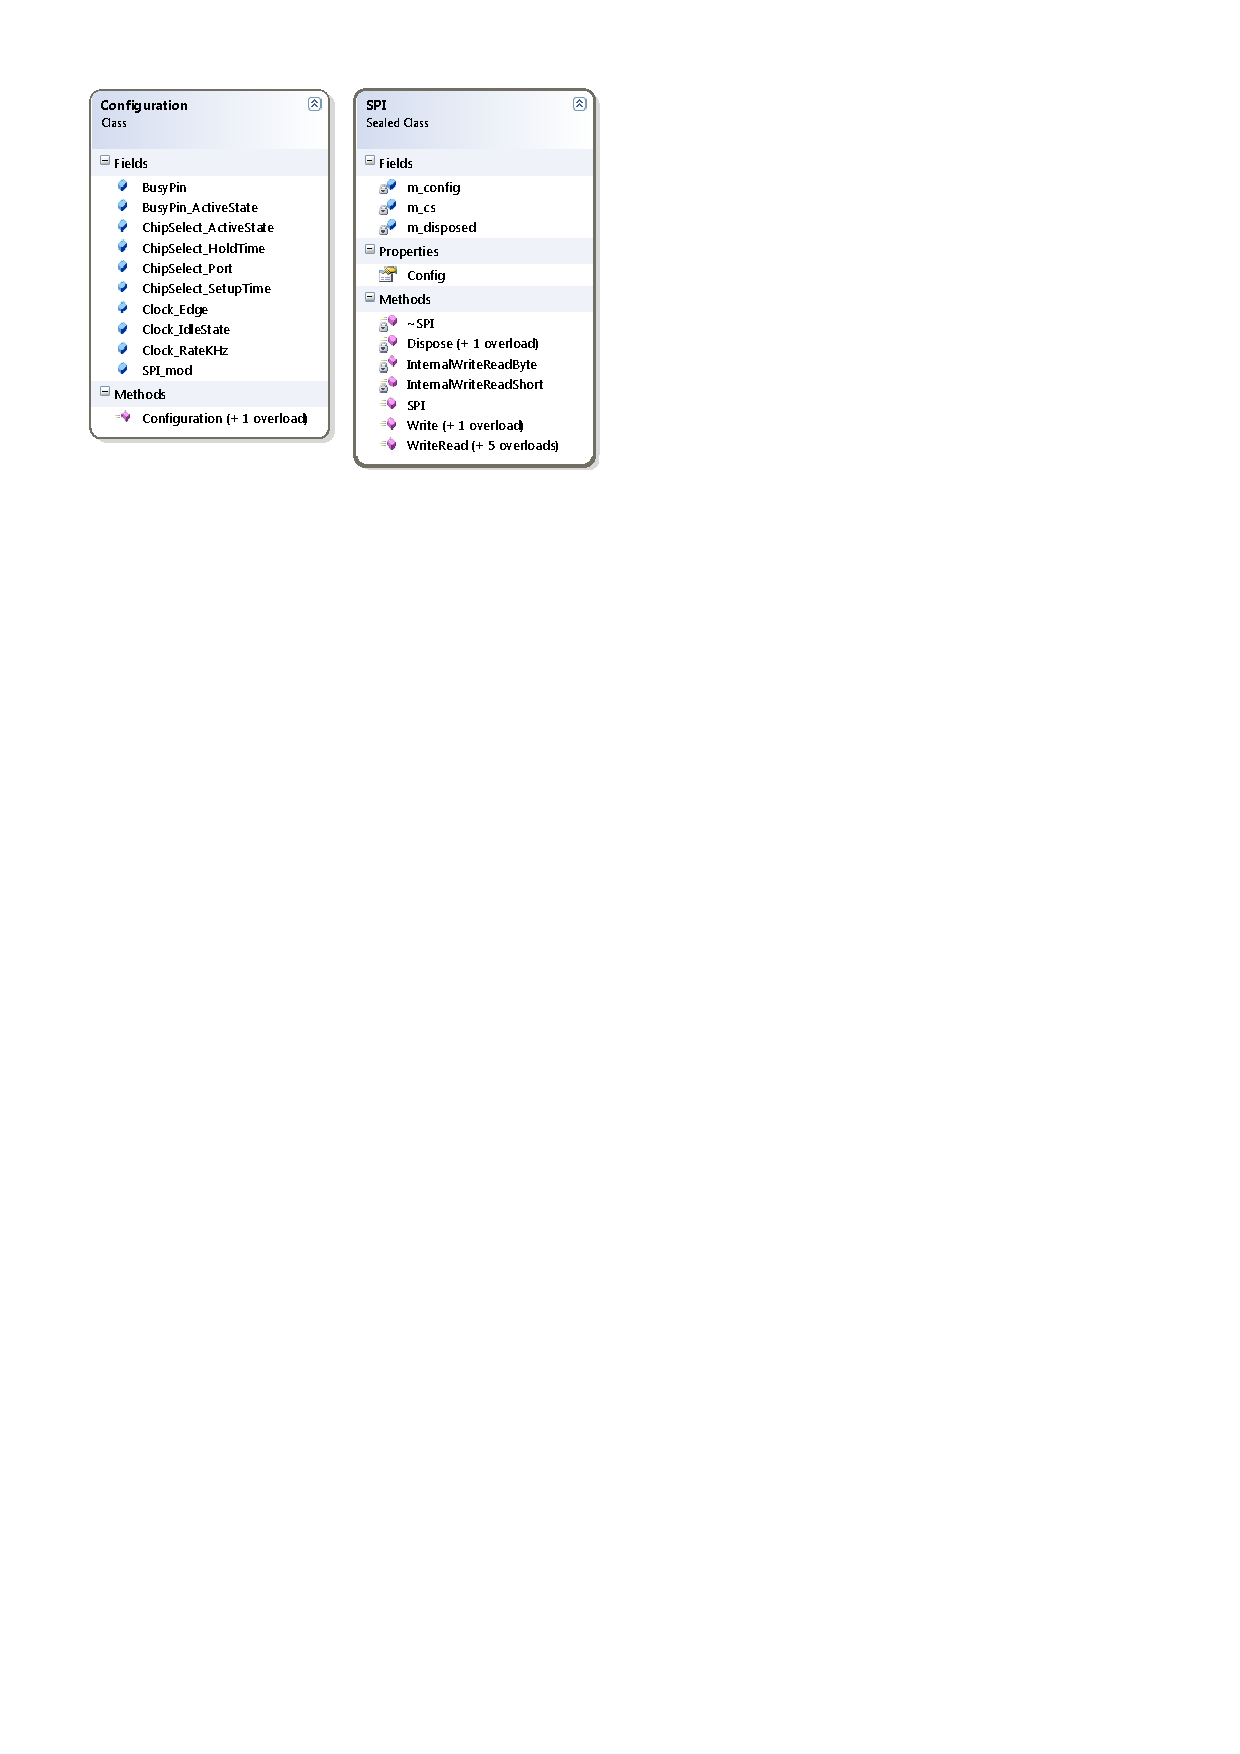
\includegraphics[scale=1]{pictures/iosharp/spi-uml}
  \caption{UML representation of the SPI Configuration Class (Left) and the SPI Port (Right) \label{fig:spi-uml}}
\end{center}\end{figure}

In order to pass the configuration to the library, the configuration object is converted to a struct which its variables are the same as the struct from the header file of the library. This struct will be the one that is passed to the C library.
\\
The code shown below corresponds to the header file and represents the struct that will be interchanged between the two languages.

\begin{lstlisting}[language=C, caption={IOSharp.h - spi\_config struct}]
typedef struct spi_config
{
  int mode;
  uint32_t speed;
  int cs_change;
  uint16_t delay;
} SPI_CONFIG;
\end{lstlisting}

The listing below represents the C\# implementation of the C struct used for the pin configuration, it contains the same parameters as the C version and also implements a constructor which simplifies the conversion between the Configuration class and this structure, the important thing in this case is the
\\
\verb![StructLayout(LayoutKind.Sequential, CharSet = CharSet.Unicode)]!. This attribute is used by the P/Invoke to know how the marshalling must be done when is passed to the library.

\begin{lstlisting}[language=CSharp, caption={SPI.cs - spi\_config struct}]
[StructLayout(LayoutKind.Sequential, CharSet = CharSet.Unicode)]
public struct spi_config {
    public int mode;
    public uint speed;
    public int cs_change;
    public ushort delay;

    public spi_config(Configuration config) {
        this.cs_change = (config.ChipSelect_ActiveState) ? 1 : 0;
        this.delay = (ushort) config.ChipSelect_HoldTime;

        if (config.Clock_Edge && !config.Clock_IdleState)
            this.mode = 0;
        else if (!config.Clock_Edge && !config.Clock_IdleState)
            this.mode = 1;
        else if (config.Clock_Edge && config.Clock_IdleState)
            this.mode = 2;
        else
            this.mode = 3;
        this.speed = config.Clock_RateKHz * 1000;
    }
}
\end{lstlisting}

It is interesting to remark that the \gls{TX}/\gls{RX} buffers are not returned from C to C\# but the buffers have been read and written so C takes the pointer of that buffer, which is the same as the C\# and then writes or reads the information from there. 

\subsection{UART}\label{SS:IOSharp-UART}
UART is a really simple protocol that uses an asynchronous serial communication between two devices. As figure \ref{fig:uart-modules} shows, each device have two ports which are the \gls{TX} for transmissions and \gls{RX} for receptions. The transmission port must be connected to the reception port on the other device. Both devices must share the ground.

\begin{figure}[H]\begin{center}
 \centering
  \captionsetup{justification=centering}
  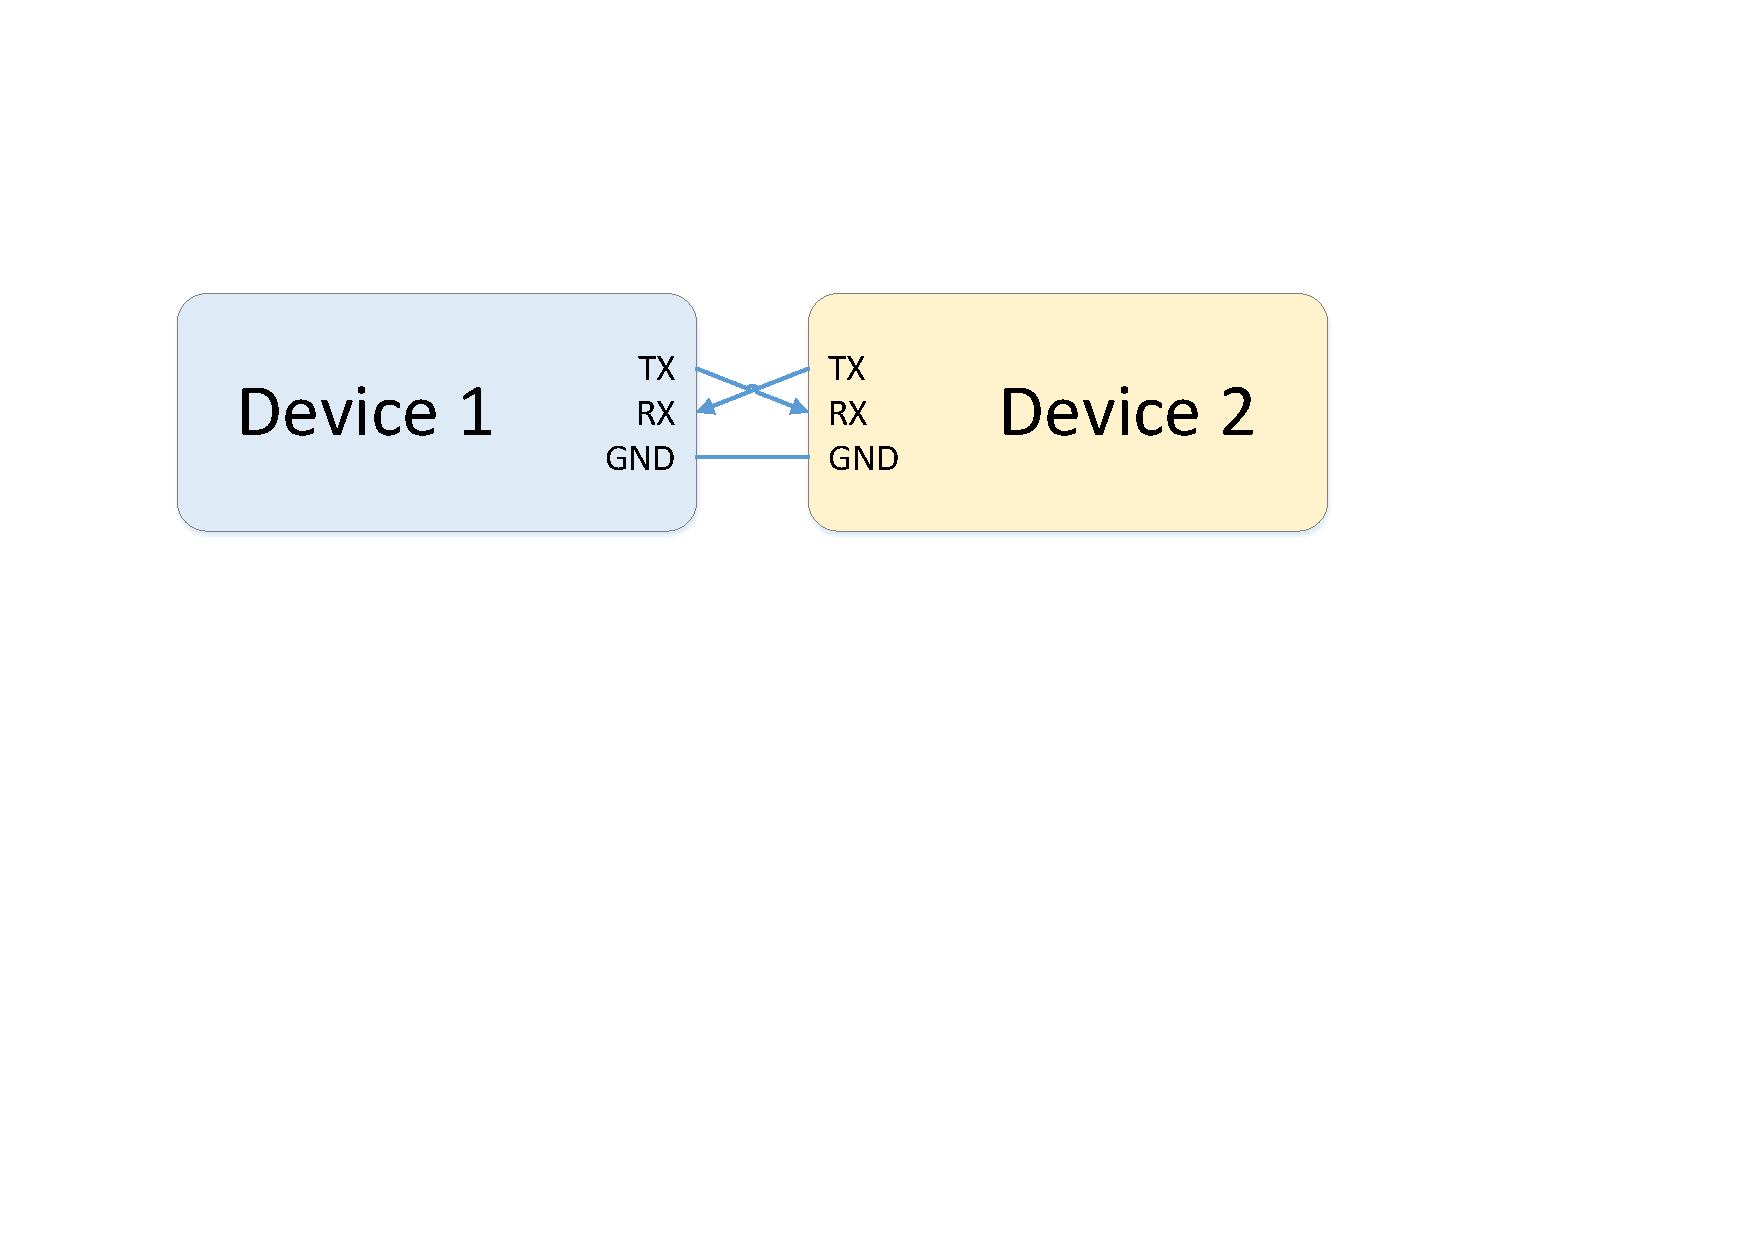
\includegraphics[scale=0.60]{pictures/iosharp/uart-modules}
  \caption{UART communication schema\label{fig:uart-modules}}
\end{center}\end{figure}

Unlike the above features which were not implemented on the standard .NET Framework the UART it is with also the same name and in the namespace, so this is problematic in case of a class reimplementation if maintaining the original namespace is desired.
\\
First of all and trying to avoid a new implementation of a SerialPort the classes from the Micro Framework and the .NET Framework were compared. After doing this it was realised that the two classes were so similar that IOSharp did not require a new reimplementation. The reason of avoiding a new implementation is due to two reasons, the first one is that any reuse of code is better rather than writing again the same feature, and considering that the communications between devices must be really well done, and .NET Framework is much more stable and tested than a code written from scratch. The other reason of this choose is that although the .NET Framework class is not exactly as the Micro Framework class, it has all the required methods that are needed for HomeSense.

\begin{figure}[H]\begin{center}
 \centering
  \captionsetup{justification=centering}
  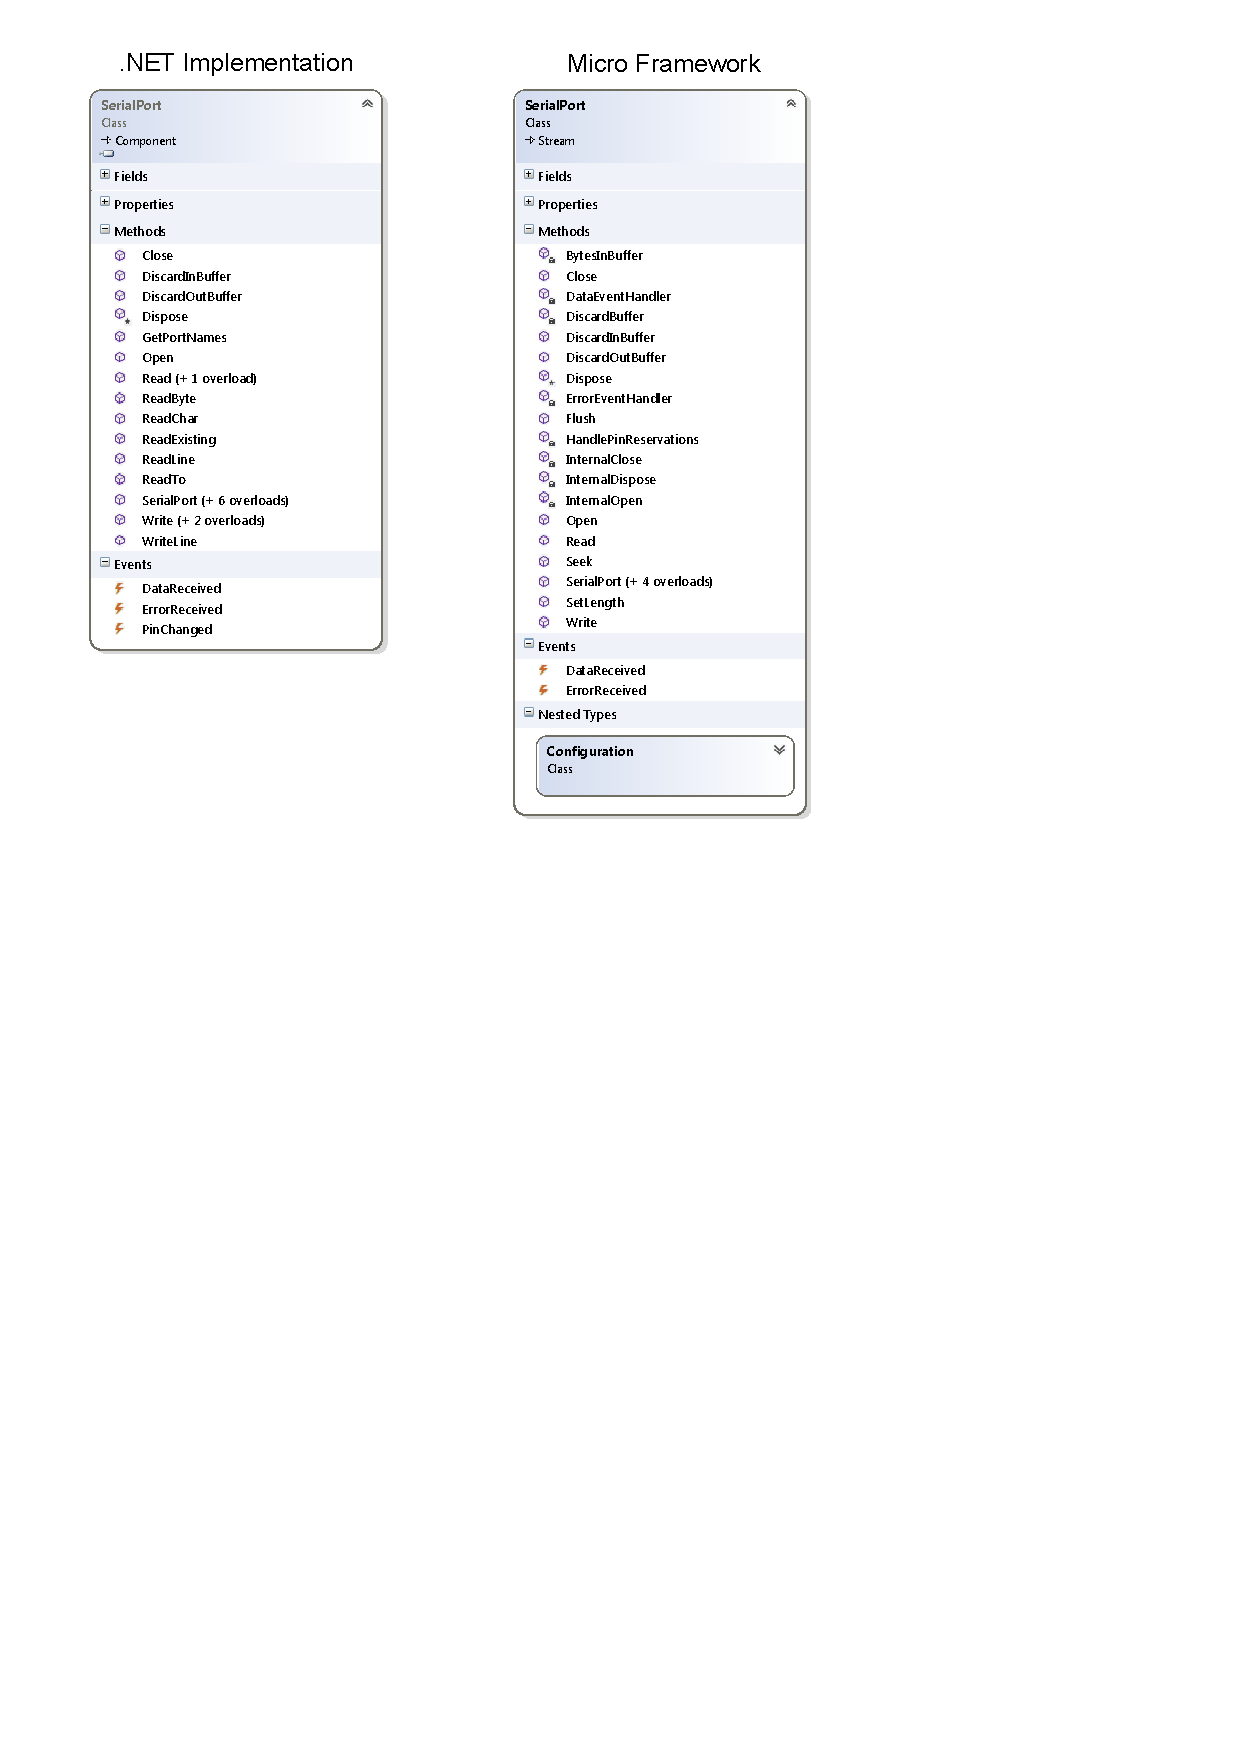
\includegraphics[scale=1]{pictures/iosharp/serialport-uml}
  \caption{UML SerialPort representation of the original .NET Framework (Left) and .NET Micro Framework (Right)\label{fig:serialport-uml}}
\end{center}\end{figure}

Is important to remark that IOSharp in Linux runs on Mono implementation of the .NET Framework classes, and in this case the SerialPort class has some disadvantages on Mono version, basically it does not support the \verb!DataReceived! or \verb!ErrorReceived! events because the functions have not been implemented on its internal runtime.

\section{Port Mapping}\label{S:Port-Mapping}
Although IOSharp is a cross-platform library some features require a specific configuration when deploying in different boards. Every board has its own port mapping and naming so it is necessary to have a specific library to describe that board.
\\
This is similar to the \gls{HAL} and \gls{PAL} concept:
\begin{itemize}
\item \textbf{HAL:} Hardware Abstraction Layer. In this case Linux acts as a HAL offering simple APIs to use features likes the kernel driven SPI device or the GPIO exposed in the SYSFS.
\item \textbf{PAL:} Platform Abstraction Layer. Is the library that must be implemented in order to exploit the HAL functionalities. In this case, the Raspberry Pi requires a library to remap the GPIO pins or the SPI device to the name that the HAL uses.
\end{itemize}

\subsection{HardwareProvider}\label{SS:HardwareProvider}
In fact, the original Micro Framework supports a hardware descriptor which represents the \gls{PAL} of the Raspberry Pi and is called \verb!HardwareProvider!. Raspberry Pi is the target platform for this project so a hardware descriptor was written, below are represented the pins of the Raspberry Pi, on the left the revision 1.0 and on the right the revision 2.0. In the image are also shown where are the different pins used for the SPI and the \gls{I2C}.

\begin{figure}[H]\begin{center}
 \centering
  \captionsetup{justification=centering}
  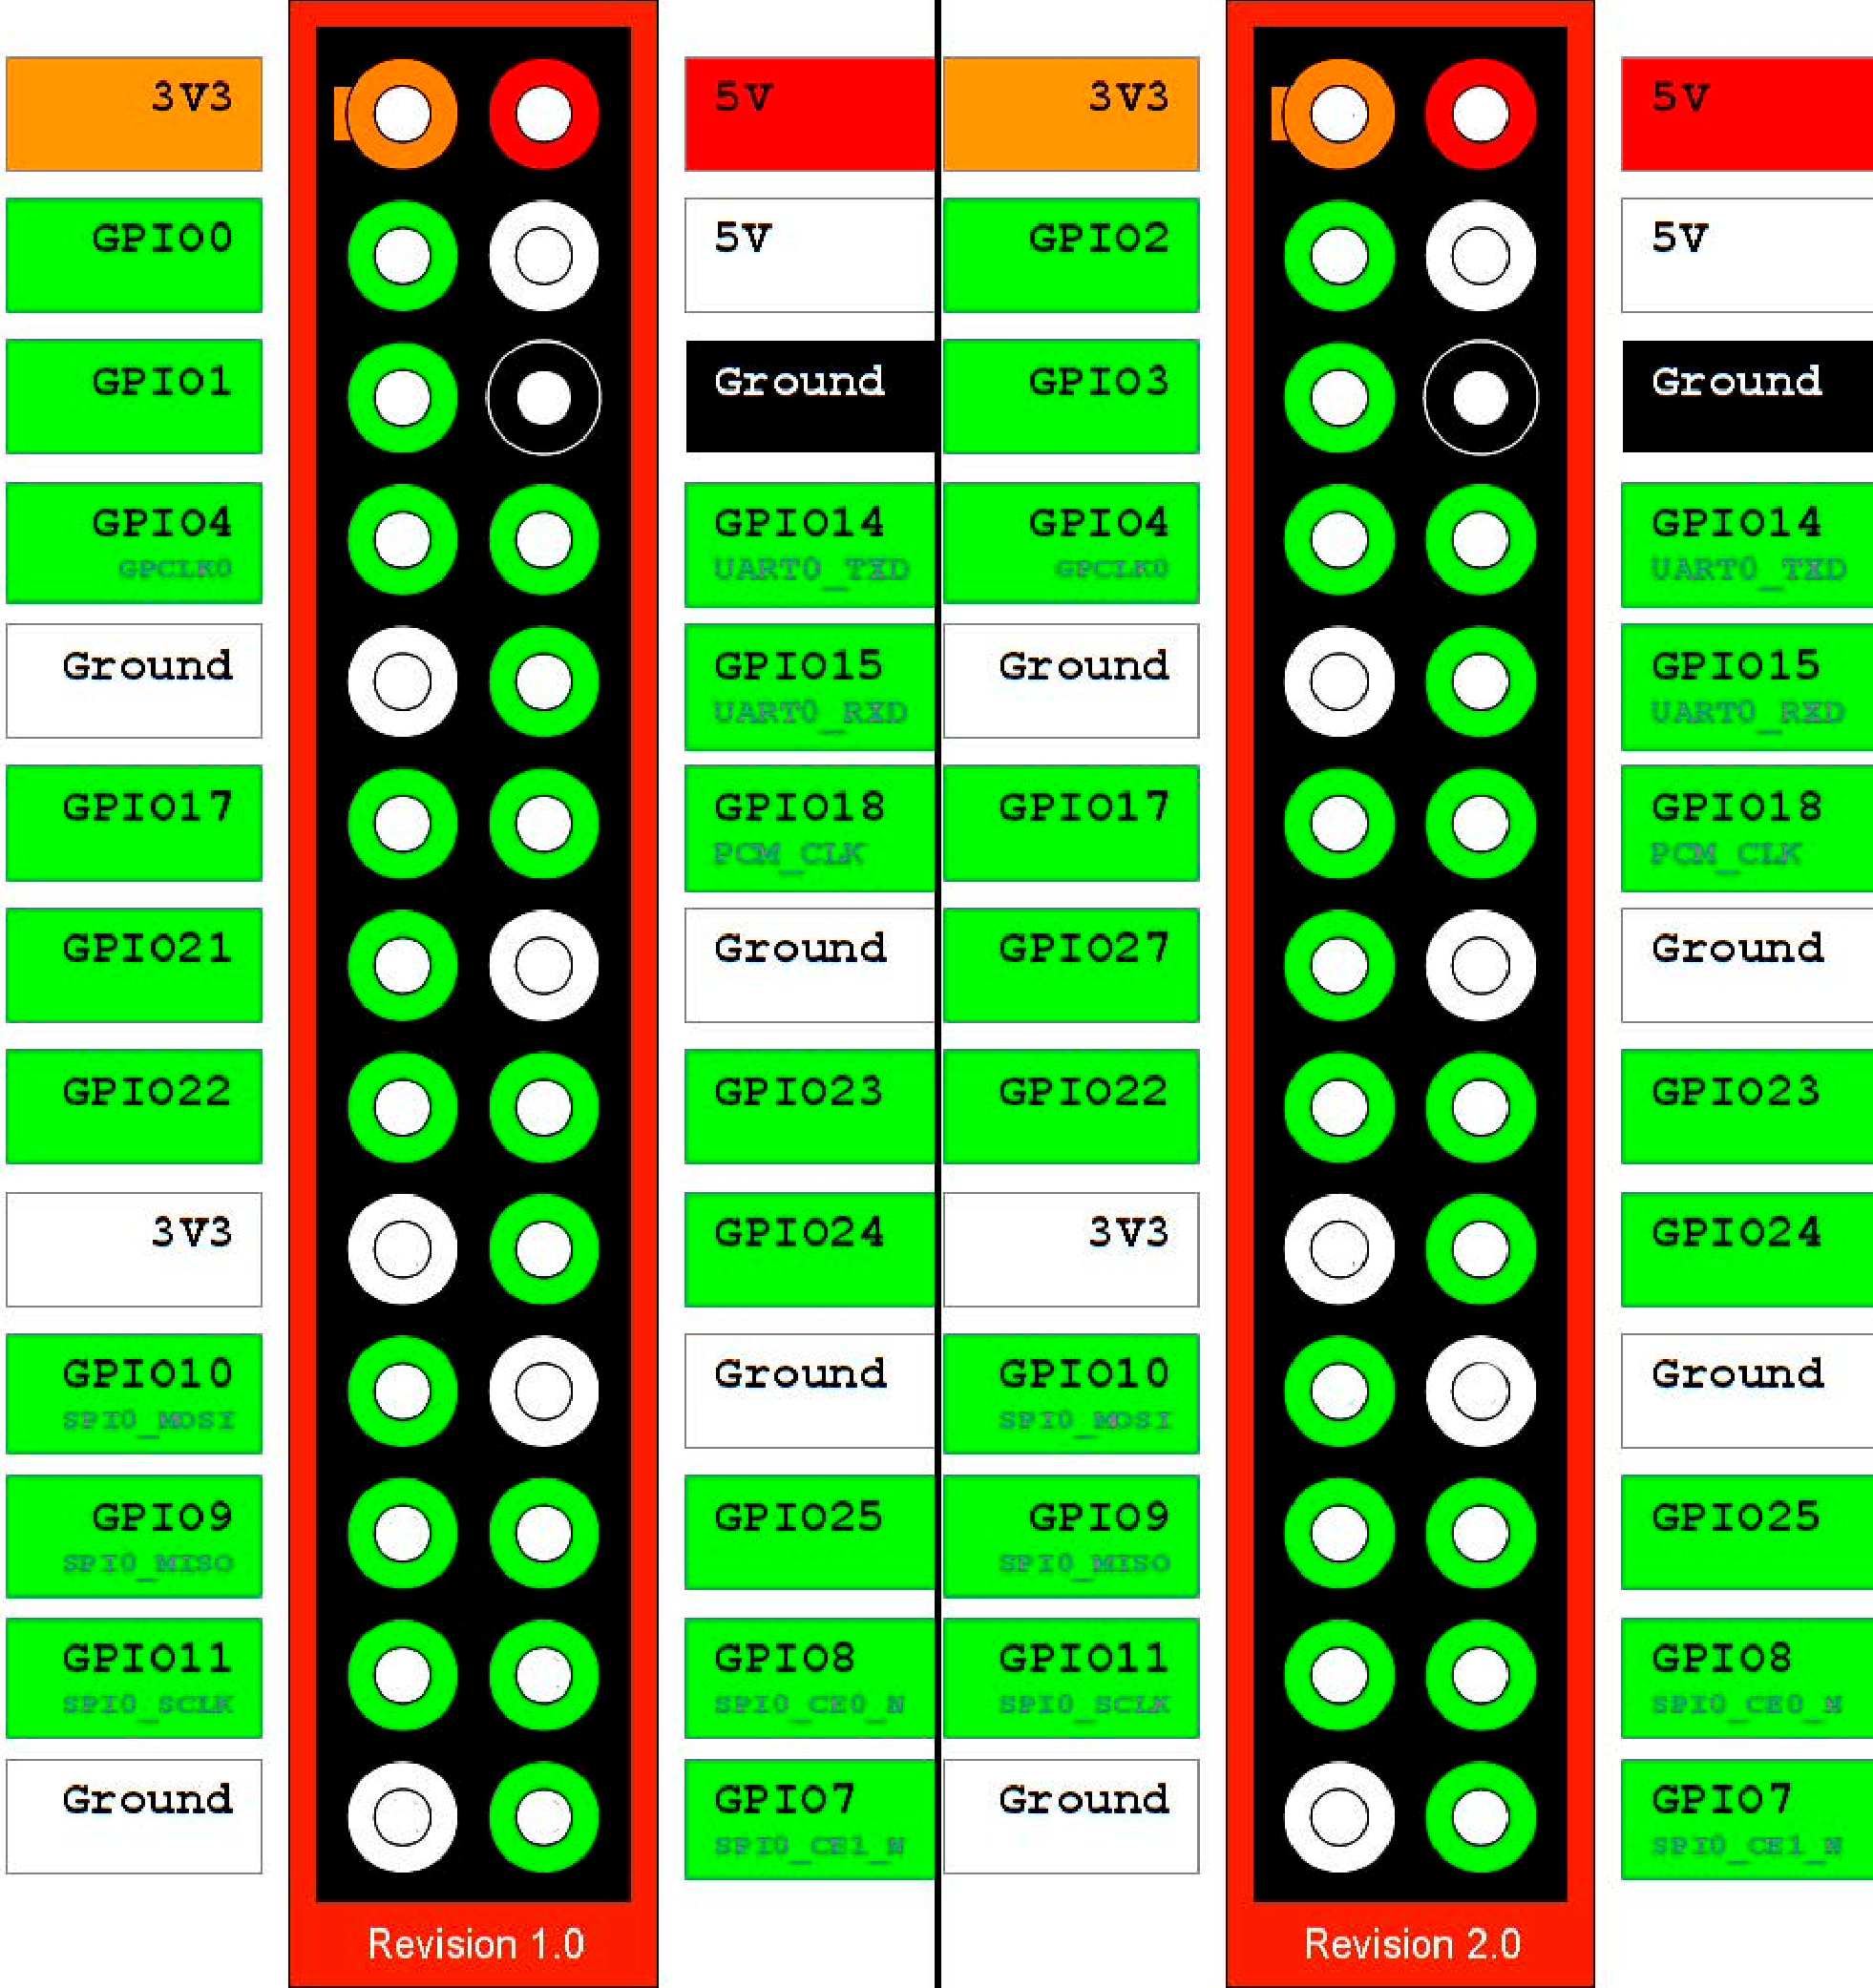
\includegraphics[scale=0.30]{pictures/iosharp/mapping-raspberrypi}
  \caption{Raspberry Pi pin mapping according to the GPIO\label{fig:mapping-rpi}}
\end{center}\end{figure}

The mapping has been divided into two classes, the first one maps the Pins so it will contain the naming according to the platform pins, in case of this thesis, both versions are mapped.
\\
The second file is used to pass the specific pins to the program, for example it configures the pins for the SPI or the UART. It is interesting to mention that in Linux the SPI and UART are known as devices so they are located under \verb!/dev/! directory. Raspberry Pi SPI device can have two slaves by using the \verb!spidev0.0! and \verb!spidev0.1!. This indicates that there are one device capable of having two slaves. The MISO, MOSI and SCLK pins are shared whereas each slave has its own chip select. In case of the UART it is also represented as a device and is named \verb!/dev/ttyAMA0! on the Raspberry Pi.